\documentclass[11pt, a4paper, titlepage]{scrartcl}

% --- SPRACHSTEUERUNG (Deutsch / Englisch) ---
% Für Deutsch: main=ngerman | Für Englisch: main=english
\usepackage[main=english, ngerman]{babel}

% --- BASIC PACKAGES ---
\usepackage[utf8]{inputenc}
\usepackage[T1]{fontenc}
\usepackage{lmodern}
\usepackage{geometry}
\geometry{left=2.5cm, right=2.5cm, top=2.5cm, bottom=3cm}
\usepackage{microtype}
\usepackage{graphicx}
\usepackage{pdfpages}
\usepackage{booktabs} % Für Tabellen
\usepackage{caption}
\usepackage{subcaption}

% --- MATHEMATIK & SI-EINHEITEN ---
\usepackage{amsmath, amssymb, mathtools}
\usepackage{siunitx}

% SI-Konfiguration an Sprache anpassen
\iflanguage{ngerman}{
    \sisetup{locale = DE, separate-uncertainty = true, per-mode = fraction}
}{
    \sisetup{locale = US, separate-uncertainty = true, per-mode = fraction}
}

% --- HIGHLIGHT-BOXEN FÜR ERGEBNISSE ---
\usepackage[most]{tcolorbox}
\newtcolorbox{resultbox}[1][]{
    enhanced,
    colback=blue!5!white,
    colframe=blue!75!black,
    fonttitle=\bfseries,
    title=#1,
    arc=2mm,
    boxrule=1pt,
    drop shadow
}

% --- CODE-FORMATIERUNG (PYTHON) ---
\usepackage{listings}
\usepackage{xcolor}

\definecolor{codegreen}{rgb}{0,0.6,0}
\definecolor{codegray}{rgb}{0.5,0.5,0.5}
\definecolor{codepurple}{rgb}{0.58,0,0.82}
\definecolor{backcolour}{rgb}{0.97,0.97,0.97}

\lstdefinestyle{pythonstyle}{
    backgroundcolor=\color{backcolour},
    commentstyle=\color{codegreen},
    keywordstyle=\color{magenta},
    numberstyle=\tiny\color{codegray},
    stringstyle=\color{codepurple},
    basicstyle=\ttfamily\footnotesize,
    breaklines=true,
    captionpos=b,
    keepspaces=true,
    numbers=left,
    showspaces=false,
    showstringspaces=false,
    showtabs=false,
    tabsize=4
}
\lstset{style=pythonstyle}

% --- LITERATURVERZEICHNIS ---
\usepackage[backend=biber, style=numeric-comp, sorting=none]{biblatex}
\addbibresource{literatur.bib}

% --- REFERENZEN & HYPERLINKS ---
\usepackage{hyperref}
\hypersetup{
    colorlinks=true,
    linkcolor=blue!80!black,
    citecolor=blue!80!black,
    urlcolor=blue!80!black
}
\usepackage[nameinlink, noabbrev]{cleveref} % Falls Protokoll auf Englisch: ngerman weglassen

% --- PROTOKOLL-INFORMATIONEN ---
\newcommand{\versuchstitel}{V11 - Introduction}
\newcommand{\praktikumstitel}{Physikalisches Anfängerpraktikum 1 (PAP1)}
\newcommand{\autor}{Oskar Kaiser}
\newcommand{\tutor}{Natalia Sycheva}
\newcommand{\datum}{\today}

\begin{document}

% --- TITELSEITE MIT INHALTSVERZEICHNIS ---
\begin{titlepage}
    \centering
    {\scshape\Large \praktikumstitel \par}
    \vspace{0.8cm}
    {\huge\bfseries \versuchstitel \par}
    \vspace{1.2cm}

    % Titelbild (Optional)
    %\begin{figure}[h!]
    %    \centering
    %    % Ersetze 'example-image' durch dein Bild (z.B. bilder/aufbau.png)
    %    \includegraphics[width=0.45\textwidth]{example-image}
    %    \caption*{Versuchsaufbau zur Bestimmung des Trägheitsmoments}
    %\end{figure}

    \vspace{0.8cm}

    \begin{tabular}{ll}
        \textbf{Autor:} & \autor \\
        \textbf{Tutor:} & \tutor \\
        \textbf{Date:} & \datum \\
    \end{tabular}

    \vfill
    \hrule
    \vspace{0.5cm}

    % Inhaltsverzeichnis direkt auf der Titelseite
    \begin{minipage}{\textwidth}
        \setcounter{tocdepth}{2}
        \tableofcontents
    \end{minipage}
    \vspace{2.5cm}
\end{titlepage}

% --- INHALTSABSCHNITTE ---
\section{Introduction}

\subsection{Goal of the experiment}
The goal of the introduction experiment was to learn basic techniques of experimenting, systematical data measuring and statistical analysis of those data. In detail the key aspects were:
\begin{itemize}
    \item Comparison of different measuringg methods to determine the period of oscillation of the spring pendulum (start/stop at mass passing the maximum elongation vs. at the zero passing) as well as determining the uncertainties of each method.
    \item Graphical calculation of the spring constant $D$ from the period of oscillation $T$ of the mass $m$.
    \item Determining the earths accaleration $g$ from the displacement $x$ of the mass $m$.
\end{itemize}

\subsection{Setup and methods of measuring}
In \cref{fig:schematischer_aufbau} one can see the setup used in the experiment.

\begin{figure}[h]
    \centering
    \includegraphics[width=0.5\textwidth]{example-image-a}
    \caption{Unfortunatly I am missing the picture of the setup (next time I will take a picture)}
    \label{fig:schematischer_aufbau}
\end{figure}

\subsection{Theoretical background}
The equation of motion of the ideal, undamped spring pendulum is:
\begin{equation}
    m \ddot{x} = -D x
    \label{eq:dgl}
\end{equation}
with $m$ being tha attached mass, $x$ the displacement from the initial position and $D$ the spring constant. The solution of the ODE for the initial condition $x(0)= x_0$ is given by a cosine function:
\begin{equation}
    x(t) = x_0 \cos(\omega t) \quad \text{mit} \quad \omega = \sqrt{\frac{D}{m}}
    \label{eq:loesung}
\end{equation}
From the relation $\omega = \frac{2\pi}{T}$ one gets the oscillation period $T$:
\begin{equation}
    T = 2\pi \sqrt{\frac{m}{D}}
    \label{eq:periodendauer}
\end{equation}
Squaring equation \ref{eq:periodendauer} yields a linear relation of the form $y = a \cdot x + b$:
\begin{equation}
    T^2 = \frac{4\pi^2}{D} \cdot m
    \label{eq:t_quadrat}
\end{equation}
The slope $a = \frac{\Delta T^2}{\Delta m}$ in the $T^2$-$m$-diagramm is therefore $a = \frac{4 \pi^2}{D}$ from which one can determine the spring constant:
\begin{equation}
    D = \frac{4\pi^2}{a}
    \label{eq:federkonstante}
\end{equation}
For the displacement $x$ of the mass $m$ due to gravitational accelaration hook's law reads:
\begin{equation}
    m g = D x \iff x = \frac{g}{D} \cdot m
    \label{eq:statisch}
\end{equation}
From the slope $a' = \frac{\Delta x}{\Delta m} = \frac{g}{D}$ in the $x$-$m$-diagramm one can then finally determine the gravitational accelaration with $g = D \cdot a'$.

\section{Measurement protocol}
The original signed protocol is attached below.
% Bindet alle Seiten der PDF skaliert ein. 
% 'pagecommand={\thispagestyle{plain}}' behält Kopf-/Fußzeilen bei.
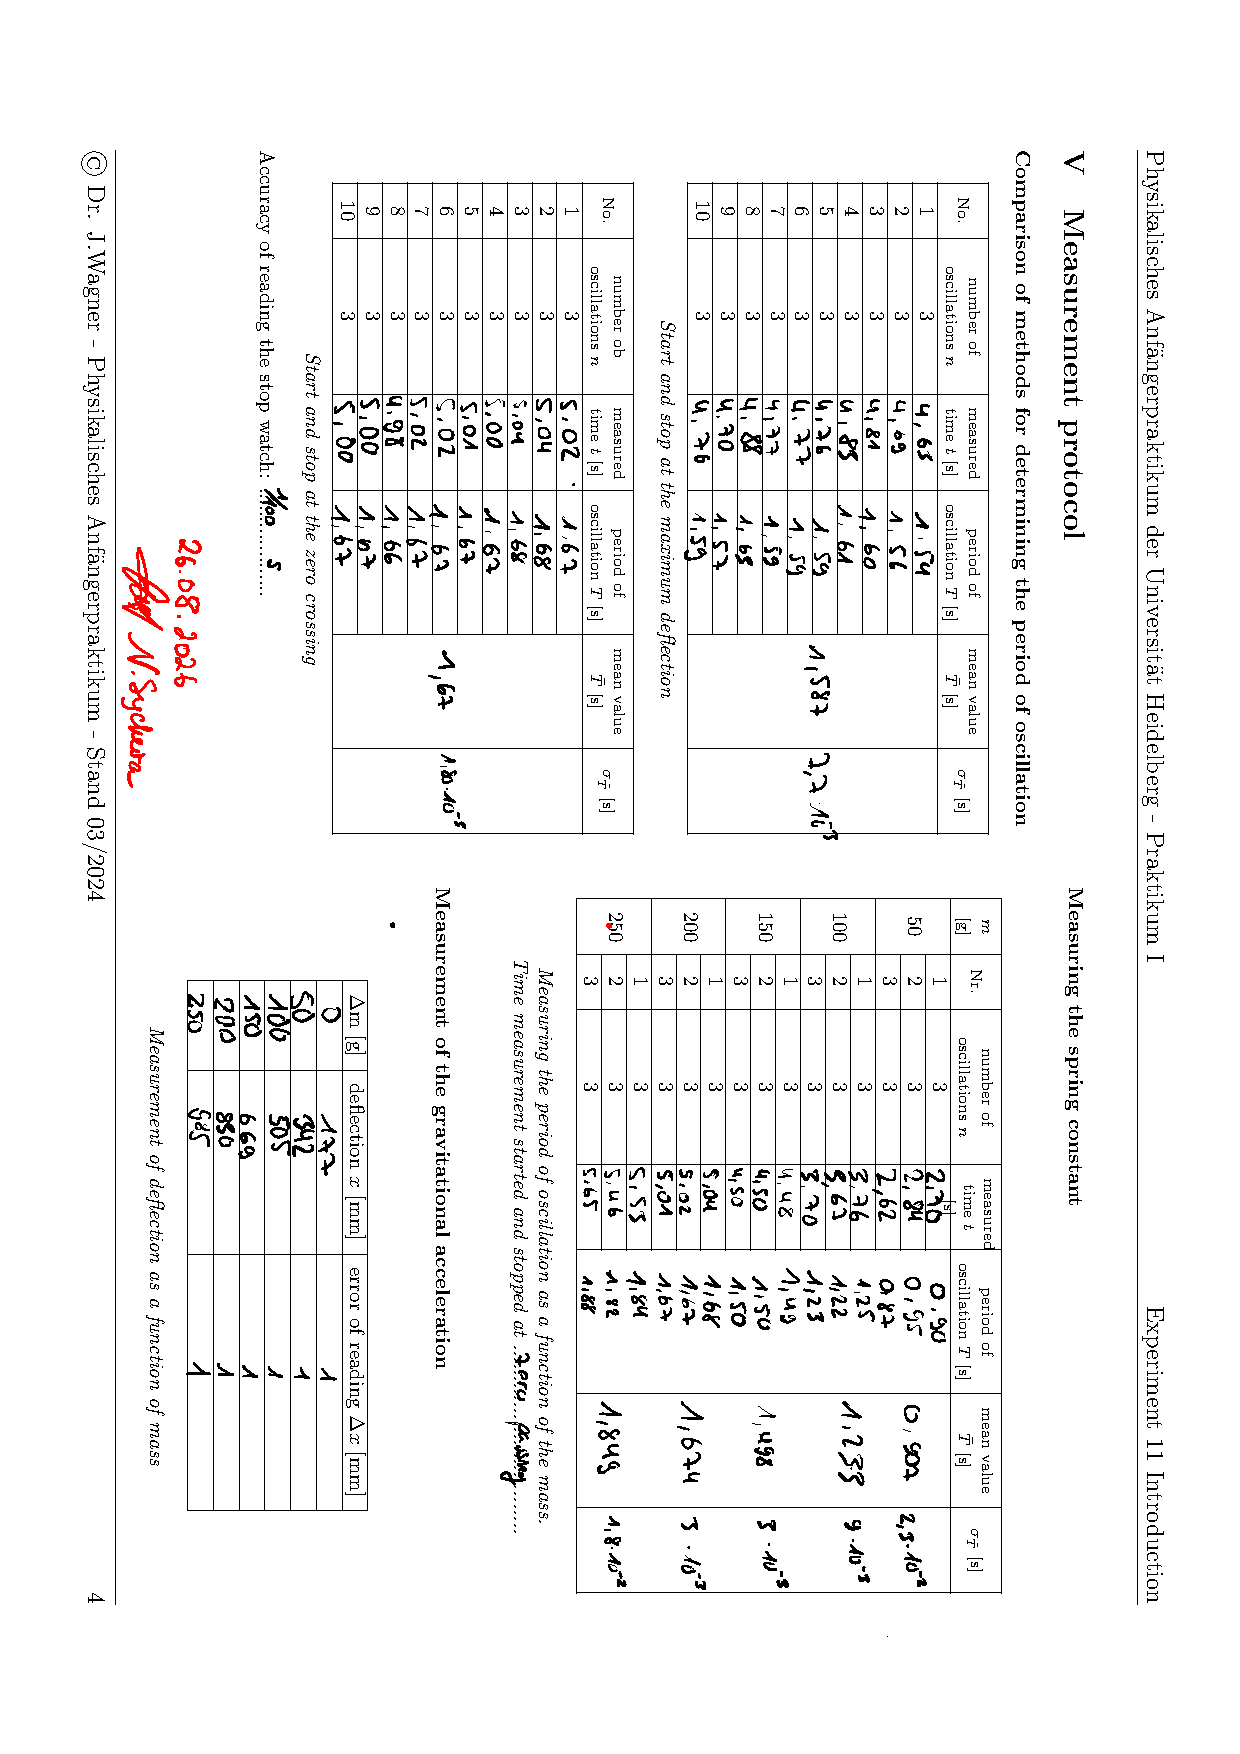
\includepdf[pages=-, scale=0.8, pagecommand={\thispagestyle{plain}}]{messprotokoll.pdf}
\section{Data analysis and results}

\subsection{Error propagation and statistical basics}
For the analysis the followin formulas have been used:
\begin{itemize}
    \item \textbf{Mean value of the osciallation period:}
    \begin{equation}
        \bar{T} = \frac{1}{n} \sum_{i=1}^{n} T_i
    \end{equation}
    
    \item \textbf{Mean error of the mean value (standard deviation):}
    \begin{equation}
        \sigma_{\bar{T}} = \sqrt{\frac{1}{n(n-1)} \sum_{i=1}^{n} (T_i - \bar{T})^2}
    \end{equation}
    
    \item \textbf{Error propagation for the squared oscillation period $T^2$:}
    As the graphical analysis of the squared oscialltion period $T^2$ is used we have to use gaussian error propagation to determine the uncertainty $\sigma_{T^2}$ of $T^2$:
    \begin{equation}
        \sigma_{T^2} = \left| \frac{\mathrm{d}(T^2)}{\mathrm{d}T} \right| \cdot \sigma_{\bar{T}} = 2 \cdot \bar{T} \cdot \sigma_{\bar{T}}
        \label{eq:fehler_t2}
    \end{equation}
\end{itemize}


\subsection{Exercise 1: Comparison of the error for the different measuring methods}
From the 10 measurement series with each measurement being $n=3$ osciallations for a mass of $m = \qty{200}{\gram}$ result in the following numbers:
\begin{itemize}
    \item \textbf{Start/stop at maximum displacement:}
    \begin{align*}
        \bar{T}_{\text{max}} &= 1{,}587\,\mathrm{s} \\
        \sigma_T &= 2{,}3 \cdot 10^{-2}\,\mathrm{s} \quad \text{(Error of individual measurement)} \\
        \sigma_{\bar{T}_{\text{max}}} &= 7{,}7 \cdot 10^{-3}\,\mathrm{s} \quad \text{(Error of the mean value)}
    \end{align*}
    
    \item \textbf{Start/stop at zero passing:}
    \begin{align*}
        \bar{T}_{\text{null}} &= 1{,}670\,\mathrm{s} \\
        \sigma_T &= 6{,}0 \cdot 10^{-3}\,\mathrm{s} \quad \text{(Error of individual measurement)} \\
        \sigma_{\bar{T}_{\text{null}}} &= 1{,}8 \cdot 10^{-3}\,\mathrm{s} \quad \text{(Error of the mean value)}
    \end{align*}
\end{itemize}

\textbf{Result:} The relativ error of the mean value with measuring at zero passing is $\frac{\sigma_{\bar{T}}}{\bar{T}} \approx 0{,}11\%$, while measuring at maximum displacement yields $\approx 0{,}49\%$. The measurement at zero passing is therefore more accurate by a factor of $4$.

\subsection{Exercise 2: Graphically determining the spring constant $D$}
In determining the spring constant we have plotted the squared oscillation amplitude $T^2$ versus the mass $m$. With the measurements and equation \eqref{eq:fehler_t2} we can determine the error bars with $\sigma_{T^2}$. The results are summarized in table \ref{tab:t2_auswertung}.
\begin{table}[h]
    \centering
    
    \begin{tabular}{c c c c c}
        \toprule
        $m$ [\unit{\kilogram}] & $\bar{T}$ [\unit{\second}] & $\sigma_{\bar{T}}$ [\unit{\second}] & $T^2$ [\unit{\second \squared}] & $\sigma_{T^2} = 2\bar{T}\sigma_{\bar{T}}$ [\unit{\second \squared}] \\
        \midrule
        0,050 & 0,907 & $2{,}3 \cdot 10^{-2}$ & 0,823 & 0,042 \\
        0,100 & 1,233 & $9{,}0 \cdot 10^{-3}$ & 1,520 & 0,022 \\
        0,150 & 1,498 & $3{,}0 \cdot 10^{-3}$ & 2,244 & 0,009 \\
        0,200 & 1,674 & $3{,}0 \cdot 10^{-3}$ & 2,802 & 0,010 \\
        0,250 & 1,849 & $1{,}8 \cdot 10^{-2}$ & 3,419 & 0,067 \\
        \bottomrule
    \end{tabular}
    \caption{Values for oscialltion period $T$ and calculated $T^2$ with error propagation.}
    \label{tab:t2_auswertung}
\end{table}
From graphical linear regression with $y = a \cdot m + b$ for $y = T^2$ we determine the slope $a$:
\begin{equation}
    a = \frac{\Delta T^2}{\Delta m} \approx \qty{13.1}{\second \squared \per \kilogram}
\end{equation}
Using best fit and worst fit line we determine the uncertainty of the slope to be $\sigma_a \approx \qty{0,5}{\second \squared \per \kilogram}$.
From equation \eqref{eq:t_quadrat} we determine $a = \frac{4\pi^2}{D}$. From that we determine the spring constant $D$ to be:
\begin{equation}
    D = \frac{4\pi^2}{a} = \frac{4\pi^2}{\qty{13.1}{\second \squared \per \kilogram}} \approx \qty{3.01}{\newton \per \meter}
\end{equation}
The error of the spring constant $\sigma_D$ is calculated via error propagation:
\begin{equation}
    \sigma_D = \left| \frac{\mathrm{d}D}{\mathrm{d}a} \right| \cdot \sigma_a = \frac{4\pi^2}{a^2} \cdot \sigma_a = \frac{4\pi^2}{\qty{13.1}{\second \squared \per \kilogram}} \cdot \qty{0.5}{\second \squared \per \kilogram} \approx \qty{0.11}{\newton \per \meter}
\end{equation}
\begin{resultbox}[Endresult: Spring constant]
    The spring used in the experiment has a spring constant of:
    \begin{equation}
        D = \qty{3.01(11)}{\newton \per \meter}
    \label{eq:ergebnis_federkonstante}
    \end{equation}
\end{resultbox}

\subsection{Exercise 3: Graphically determining the earths acceleration $g$}
The displacement $x$ in relation to the mass $m$ can be viewed as a linear function $x(m)$ and we now have to determine its slope.
\begin{table}[h!]
    \centering
    \begin{tabular}{c c c}
        \hline
        $m$ [kg] & Displacement $x$ [m] & Error $\Delta x$ [m] \\
        \hline
        0,050 & 0,177 & 0,001 \\
        0,100 & 0,342 & 0,001 \\
        0,150 & 0,505 & 0,001 \\
        0,200 & 0,669 & 0,001 \\
        0,250 & 0,850 & 0,001 \\
        \hline
    \end{tabular}
    \caption{Measurements of displacement $x$ as a function of mass $m$.}
    \label{tab:auslenkung_auswertung}
\end{table}

From best fit line $x = a' \cdot m + x_0$ we can determine $a'$ to he:
\begin{equation}
    a' = \frac{\Delta x}{\Delta m} \approx 3{,}36\,\mathrm{\frac{m}{kg}} \quad \text{mit einem abgeschätzten Steigungsfehler } \sigma_{a'} \approx 0{,}04\,\mathrm{\frac{m}{kg}}
\end{equation}
From hooks law ($x = \frac{g}{D} \cdot m$) we determine the slope to be $a' = \frac{g}{D}$. From that we get the gravitational accelaration $g$ to be:
\begin{equation}
    g = D \cdot a' = \qty{3.01}{\newton \per \meter} \cdot \qty{3.36}{\meter \per \kilogram} \approx \qty{10.13}{\meter \per \second \squared}
\end{equation}
As $D$ as well as $a'$ have an error we need to calculate the the resulting error $\sigma_g$ via gaussian error propagation for two variables:
\begin{align}
    \sigma_g &= \sqrt{ \left( \frac{\partial g}{\partial D} \cdot \sigma_D \right)^2 + \left( \frac{\partial g}{\partial a'} \cdot \sigma_{a'} \right)^2 } \\
             &= \sqrt{ (a' \cdot \sigma_D)^2 + (D \cdot \sigma_{a'})^2 } \\
             &= \sqrt{ (3{,}365 \cdot 0{,}06)^2 + (3{,}041 \cdot 0{,}04)^2 } \approx 0{,}24\,\mathrm{\frac{m}{s^2}}
\end{align}


\begin{resultbox}[Endresult: Gravitational acceleration]
    \begin{equation}
        g = (10{,}2 \pm 0{,}2)\,\mathrm{\frac{m}{s^2}}
    \end{equation}
\end{resultbox}






\section{Conclusion and discussion}

\subsection{Comparison with real values}
Compared to the real value for $g$ we are slightly off
%\section{Anhang}

\subsection{Python-Code zur Datenauswertung}
Der folgende Code wurde zur Berechnung der Regressionen und Fehlerfortpflanzung verwendet:

\begin{lstlisting}[language=Python, caption={Auswertungsskript für Auslenkung und Trägheitsmoment}]
import numpy as np
import matplotlib.pyplot as plt

# Messdaten laden
m = np.array([0.10, 0.20, 0.50]) # kg
s = np.array([2.345, 4.690, 11.725]) # cm

# Lineare Regression
p, cov = np.polyfit(m, s, 1, cov=True)
print(f"Steigung: {p[0]:.4f} +/- {np.sqrt(cov[0][0]):.4f}")
\end{lstlisting}

% --- LITERATURVERZEICHNIS ---
\printbibliography[heading=bibintoc]

\end{document}